%------------------------------------------------------------------------------
% Author(s):
% Brad Bachu, Varaun Ramgoolie
%
% Copyright:
%  Copyright (C) 2020 Brad Bachu, Arjun Mohammed, Varaun Ramgoolie, Nicholas Sammy
%
%  This file is part of Applied-Mathematics-Unit2 and is distributed under the
%  terms of the MIT License. See the LICENSE file for details.
%
%  Description:
%     Year: 2014
%     Module: 3
%     Question: 5*
%------------------------------------------------------------------------------

%------------------------------------------------------------------------------
% 5 a
%------------------------------------------------------------------------------
	
\begin{subquestions}
	
	\subquestion
	
	We are given the displacement function of a particle, from a fixed point $O$, as it moves along a straight line.
	
	\begin{subsubquestions}
		
		\subsubquestion
		
		\rfig{2014:q5*:SGraph1} shows the displacement-time graph of the particle.
		\begin{figure}[H]
			\begin{center}
				\includegraphics{../2014/figures/DispGraph-2014-q5-a-i}
				\caption{\label{2014:q5*:SGraph1} Displacement-time graph of the particle's motion.}
			\end{center}
		\end{figure}
		
		It is useful to interpret the different regions of this graph so that we can get a stronger understanding of the motion of the particle. Using the given $s(t)$, we can see that the roots of the graph (points at which $s=0$) must occur when $t=2$ and $t=6$. We can also notice that the graph is a `U' shape as the graph of $s(t)$ is quadratic with a positive $t^2$ coefficient. 
		
		For $0 \leq t < 2$, we can see that the displacement of the particle is positive, from the fixed point $O$. For $2 < t < 6$, the displacement is negative and for $t>6$, the particle's displacement is positive. 
		
		We know that the gradient of a displacement-time graph is equivalent to velocity of the particle at any point in time. Therefore, we can notice that the velocity of the particle is negative for $12 \leq t < 4$ and positive for $t>4$ (this is indicative of the particle moving in the negative direction for $0 \leq t < 4$ and in a positive direction for $t>4$). 
		
		At $t=4$, we see that the motion of the particle seems to `turn around' and the velocity changes from negative to positive. 
		
		%------------------------------------------------------------------------------
		
		\subsubquestion
		
		\begin{subsubsubquestions}
			
			\subsubsubquestion
			
			\textbf{\textit{Simplify and Diagram:}} \\ \\
			
			\begin{figure}[H]
				\begin{center}
					\includegraphics{../2014/figures/DispGraph2-2014-q5-a-ii}
					\caption{\label{2014:q5*:SGraph2} Displacement-time graph of particle.}
				\end{center}
			\end{figure}
			
			We want to find the distance traveled from $t=0$ to $t=5$ (green line in \rfig{2014:q5*:SGraph2}). From \rfig{2014:q5*:SGraph1}, we know that the graph changes direction at $t_m=4$. This means that, in order to find the total distance traveled, we have to consider two pieces of the graph separately and sum their results. We do this because, in the period of time given, the particle moves in opposite directions (which increases the change in distance but decreases the change in displacement). We will consider $0 \leq t < 4$ and $4 < t < 5$ separately.
			
			
			
			\textbf{\textit{Represent Mathematically:}} \\ \\
			We will first represent the distance between $t=0$ and $t=4$ as,
			\begin{align}
				\text{Distance}_{t=0 \rightarrow 4} & = \text{Final Displacement - Initial Displacement} \nn \\
				& = |s(4)-s(0)| \,.  \label{2014:q5*:Seqn1}
			\end{align}
			
			We will then represent the distance between $t=4$ and $t=5$ as,
			\begin{align}
				\text{Distance}_{t=4 \rightarrow 5} & = \text{Final Displacement - Initial Displacement} \nn \\
				& = |s(5)-s(4)| \,.  \label{2014:q5*:Seqn2}
			\end{align}
			
			As we have split the distance that we want to find into 2 sections, we must represent this as,
			\begin{equation}
				\text{Distance}_{t=0 \rightarrow 5} = \text{Distance}_{t=0 \rightarrow 4} + \text{Distance}_{t=4 \rightarrow 5} \,. \label{2014:q5*:Seqn3}
			\end{equation}
			
			The modulus signs in the expressions are used to ensure that our answer is positive. Negative distance does not make sense (but negative displacement does).
			
			
			
			\textbf{\textit{Solve and Evaluate:}} \\ \\
			Substituting our values into \req{2014:q5*:Seqn1}, we get,
			\begin{align}
				\text{Distance}_{t=0 \rightarrow 4} & = |s(4)-s(0)| \nn \\
				& = |-4-12| \nn \\
				& = |-16| \nn \\
				& = 16 \text{m} \,.
			\end{align}
			
			For our second section, we will use $t_2=5$ and $t_m=4$ and \req{2014:q5*:Seqn2} as,
			\begin{align}
				\text{Distance}_{t=4 \rightarrow 5} & = |s(5)-s(4)| \nn \\
				& = |((5-2)(5-6)) -(-4)| \nn \\
				& = |(3)(-1)-(-4)| \nn \\
				& = |-3+4| \nn \\
				& = |1| \nn \\
				& = 1 \text{m} \,.
			\end{align}
			
			Finally, using \req{2014:q5*:Seqn3}, we get that,
			\begin{align}
				\text{Distance}_{t=0 \rightarrow 5} & = \text{Distance}_{t=0 \rightarrow 4} + \text{Distance}_{t=4 \rightarrow 5} \nn \\
				& = 16 + 1 \nn \\
				& = 17 \text{m} \,.
			\end{align}
			
			%------------------------------------------------------------------------------
			
			\subsubsubquestion
			
			\textbf{\textit{Simplify and Diagram:}} \\ \\
			We want to find the average velocity over $t=0$ to $t=5$. In this case, we need to find the displacement over this period. Then, in order to find the average velocity, we divide that displacement by the time taken (as per the definition of average velocity). \\
			
			
			
			\textbf{\textit{Represent Mathematically:}} \\ \\
			To find the displacement from $t=0$ to $t=5$, we do not have to consider any changing directions. We can directly find the displacement using,
			\begin{align}
				s_{t=0 \rightarrow 5} & = \text{Final Displacement - Initial Displacement} \nn \\
				& =  s(5)-s(0) \,. \label{2014:q5*:Seqn4} 
			\end{align}
			
			Using the definition of average velocity, we can find that,
			\begin{align}
				v_{avg(t=0 \rightarrow 5)} & = \frac{s_{t=0 \rightarrow 5}}{\Delta t} \nn \\
				& = \frac{s_{t=0 \rightarrow 5}}{5-0} \,. \label{2014:q5*:Seqn5}
			\end{align}
			
			
			
			\textbf{\textit{Solve and Evaluate:}} \\ \\
			Using \req{2014:q5*:Seqn4}, we can find,
			\begin{align}
				s_{t=0 \rightarrow 5} & =  s(5)-s(0) \nn \\
				& = -3 - 12 \nn \\
				& = -15 \text{m} \,.
			\end{align}
			
			Using \req{2014:q5*:Seqn5}, we get that,
			\begin{align}
				v_{avg(t=0 \rightarrow 5)} & =\frac{s_{t=0 \rightarrow 5}}{5-0} \nn \\
				& = \frac{-15}{5-0} \nn \\
				& = -3 \text{ms}^{-1} 
			\end{align}
			
			%------------------------------------------------------------------------------
			
			\subsubsubquestion
			
			\textbf{\textit{Simplify and Diagram:}} \\ \\
			We are given that the displacement of the particle, $s(t)$, is a function of time. By definition, we know that the velocity of the particle, $v(t)=\frac{d}{dt}(s(t))$. Therefore, we can find the derivative of $s(t)$ and find the value of $t$ which makes that derivative 0.
			
			
			
			\textbf{\textit{Represent Mathematically:}} \\ \\
			By differentiating $s(t)$, we get,
			\begin{align}
				v(t) & = \frac{d}{dt}(s(t)) \nn \\
				     & = \frac{d}{dt}(t^2-8t+12) \nn \\
				     & = 2t - 8 \,.
			\end{align}
		
		
		
			\textbf{\textit{Solve and Evaluate:}} \\ \\
			We can now set $v(t)$ equal to 0 and find the corresponding value of $t$.
			\begin{align}
				v(t) = 2t-8 & = 0 \nn \\
				       2t & = 8 \nn \\
				       \implies t & = 4\text{s} \,.
			\end{align}
			
			Thus, we get that, at $t=4$, the velocity of the particle is 0 (stationary).
			
			In addition to this, another intuition that can motivate this solution is that the quadratic of $s(t)$ must be symmetric about its minimum point. As we have already discussed in the first solution, we know that this minimum point must be the point where the velocity is 0. From $s(t)=(t-2)(t-6)$, we can see that the roots are $t=2$ and $t=6$. Therefore, the minimum point must occur at the midpoint of these roots which means that the midpoint occurs at $t=\frac{2+6}{2}=4$.
		\end{subsubsubquestions}
		
	\end{subsubquestions}

%------------------------------------------------------------------------------
% 5 b
%------------------------------------------------------------------------------

\begin{subsubquestions}
	
	\subsubquestion
	
	\textbf{\textit{Sketch and Translate:}} \\ \\
	We are given a series of forces which act on a particle, we will call $O$, with mass, $m$. \rfig{2014:q55:Force1} shows the forces acting on the particle.
	\begin{figure} [H]
		\begin{center} 
			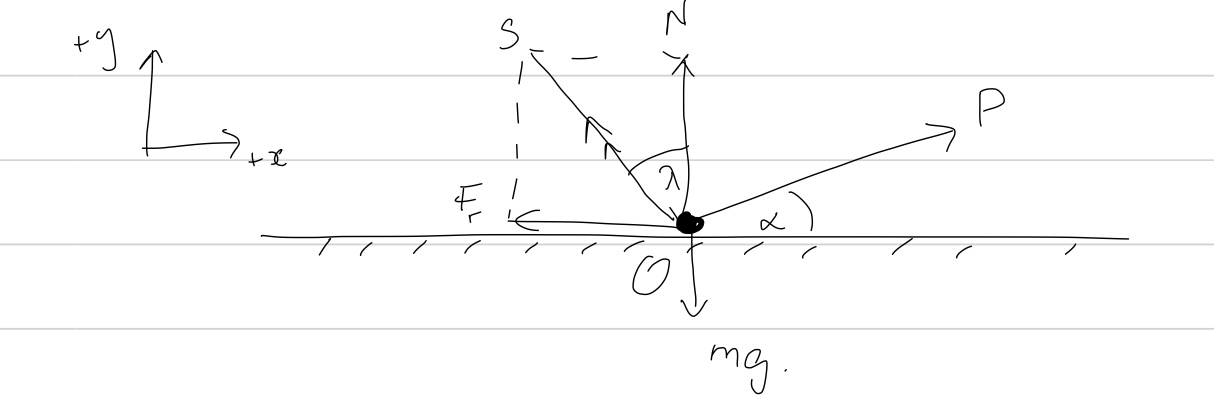
\includegraphics[scale=0.25]{../2014/figures/2014q55Sketch}
			\caption{\label{2014:q55:Force1} Diagram of forces on particle.}
		\end{center}
	\end{figure}
	
	Note that we have taken the positive $x$ direction to be towards the right. Therefore we've drawn the frictional force to the left. Given that the particle is just about to move, it is in (translational) equilibrium.
	%------------------------------------------------------------------------------
	
	\subsubquestion
	
	\textbf{\textit{Simplify and Diagram:}} \\ \\
	\rfig{2014:q55:Force2} shows all the forces acting on the particle.
	\begin{figure} [H]
		\begin{center} 
			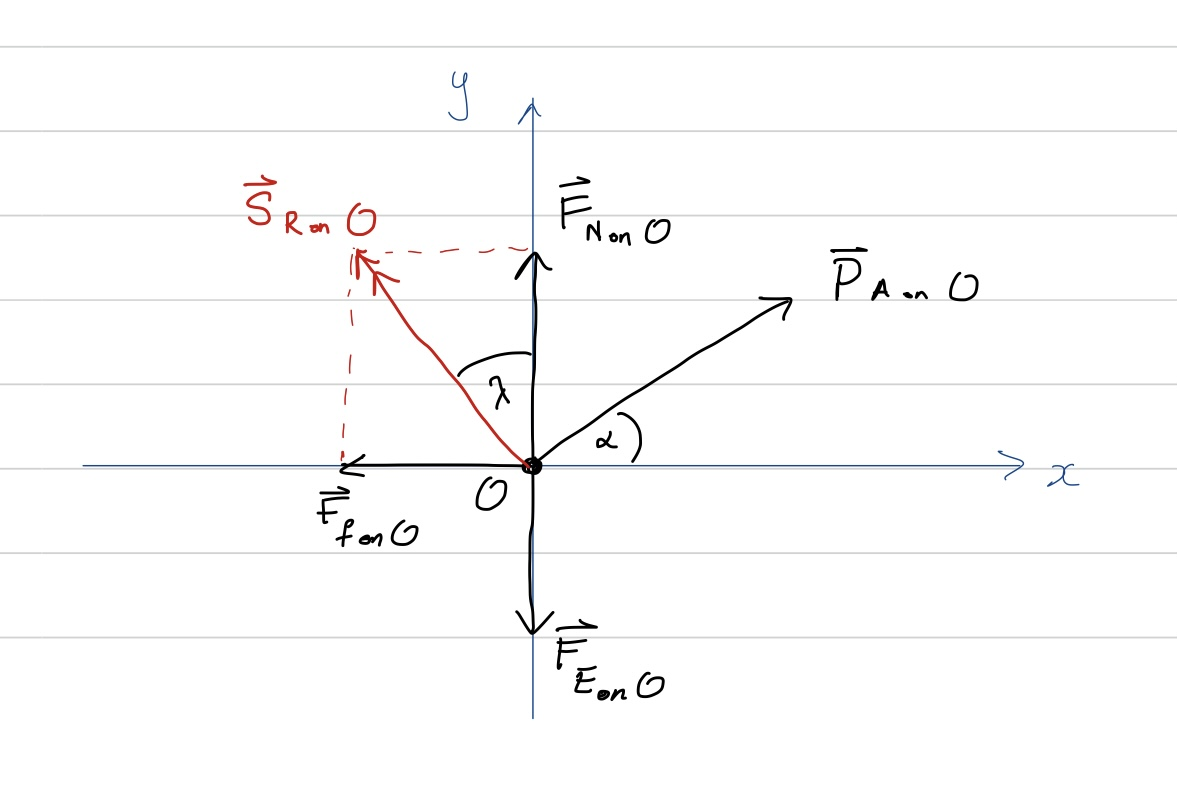
\includegraphics[scale=0.25]{../2014/figures/2014q55Diagram}
			\caption{\label{2014:q55:Force2} Diagram of forces and angles on particle.}
		\end{center}
	\end{figure}
	
	Let, 
	\begin{itemize}
		\item $\vec{F}_{fr}$ be the force of friction on $O$.
		\item $\vec{F}_{E}$ be the gravitational force of the Earth on $O$.
		\item $\vec{N}_{r}$ be the reaction force of the plane on $O$.
		\item $\vec{P}_{A}$ be the applied force on $O$.
		\item $\vec{S}_{R}$ be the resultant force of friction and the normal reaction force (as given in question) on $O$.
	\end{itemize}

	We have illustrated this in \rfig{2014:q55:Force2}.
	
	
	
	\textbf{\textit{Represent Mathematically:}} \\ \\
	To find the least value of P (which occurs when $O$ is in equilibrium,), we can represent our forces in terms of their vector components and use Newton's 2nd Law.
	
	We can consider 3 important forces,
	\begin{align}
		\vec{F}_{E} & = -mg\jhat ,\\ \nn \\
		\vec{S}_{R} & = -|\vec{S}_{R}|\sin{\lambda}\ihat +|\vec{S}_{R}|\cos{\lambda}\jhat ,\\ \nn \\
		\vec{P}_{A} & = |\vec{P}_{A}|\cos{\alpha}\ihat + |\vec{P}_{A}|\sin{\alpha}\jhat  \,.
	\end{align}

	By Newton's 2nd Law,
	\begin{align}
		m\vec{a} & = \sum{\vec{F}} \nn \\
		         & = \vec{F}_{E} + \vec{S}_{R} + \vec{P}_{A} \,.
	\end{align}

	As we know that the acceleration, $\vec{a}$, of $O$ is 0 at equilibrium, we get that,
	\begin{align}
		0\ihat + 0\jhat & = \vec{F}_{E} + \vec{S}_{R} + \vec{P}_{A} \nn \\
                        & = (|\vec{P}_{A}|\cos{\alpha} - |\vec{S}_{R}|\sin{\lambda})\ihat + (|\vec{P}_{A}|\sin{\alpha} + |\vec{S}_{R}|\cos{\lambda} - mg)\jhat \,.		
	\end{align}



	\textbf{\textit{Solve and Evaluate:}} \\ \\
	Solving the $\ihat$ component, we get,
	\begin{align}
		0 & = |\vec{P}_{A}|\cos{\alpha} - |\vec{S}_{R}|\sin{\lambda} \nn \\
		|\vec{S}_{R}|\sin{\lambda} & = |\vec{P}_{A}|\cos{\alpha} \nn \\
		|\vec{S}_{R}| & = |\vec{P}_{A}| \left(\frac{\cos{\alpha}}{\sin{\lambda}}\right) \,.
	\end{align}
	
	Solving the $\jhat$ component, we get,
	\begin{align}
		0 & = |\vec{P}_{A}|\sin{\alpha} + |\vec{S}_{R}|\cos{\lambda} - mg \nn \\
		mg & = |\vec{P}_{A}|\sin{\alpha} + |\vec{S}_{R}|\cos{\lambda} \nn \\
		 & = |\vec{P}_{A}|\sin{\alpha} + |\vec{P}_{A}|\left(\frac{\cos{\alpha}}{\sin{\lambda}}\right)\cos{\lambda} \nn \\
		 & = |\vec{P}_{A}|\left(\sin{\alpha} + \left(\frac{\cos{\alpha}}{\sin{\lambda}}\right)\cos{\lambda}\right) \nn \\
		 & = |\vec{P}_{A}|\left(\sin{\alpha} + \cos{\alpha}\left(\frac{\cos{\lambda}}{\sin{\lambda}}\right)\right) \nn \\
		 & = |\vec{P}_{A}|\left(\frac{\sin{\alpha}\sin{\lambda}+\cos{\alpha}\cos{\lambda}}{\sin{\lambda}}\right) \nn \\
		 & = |\vec{P}_{A}|\left(\frac{\cos(\alpha - \lambda)}{\sin{\lambda}}\right) \nn \\
		\implies |\vec{P}_{A}| & = \frac{mg \sin{\lambda}}{\cos(\alpha-\lambda)} \,.
	\end{align} \footnote{We use the fact that $\cos(A-B)=\cos{A}\cos{B} + \sin{A}\sin{B}$ to simplify our expression.}

	As we now have a closed form for $|\vec{P}_{A}|$ (and by extension $P$), we can work to minimize this expression. We should notice that $|\vec{P}_{A}|$ has a denominator of $\cos(\alpha - \lambda)$. This means that, in order to minimize $P$, we have to maximize this denominator. The Cosine function has a maximum value of 1 and this occurs when the argument of the function is equal to 0. This implies that the argument of $\cos(\alpha - \lambda)$ must be equal to 0. This means,
	\begin{align}
		\cos(\alpha - \lambda) & = \cos(0) \nn \\
		\implies \alpha - \lambda & = 1 \nn \\
		\implies \alpha & = \lambda \,.
	\end{align}
	
	Using this new information, we get that the minimum value of $P$ occurs when $\alpha=\lambda$ and thus,
	\begin{align}
		|\vec{P}_{A}|_{\text{min.}} & = \frac{mg\sin(180-\lambda)}{\cos(\alpha-\lambda)} \nn \\
		& = \frac{mg\sin(180-\lambda)}{\cos(0)} \nn \\
		& = mg\sin(180-\lambda) \nn \\
		& = mg\sin(\lambda) \,. \label{2014:q55:MinP}
	\end{align}

	%------------------------------------------------------------------------------
	
	\subsubquestion
	
	\textbf{\textit{Solve and Evaluate:}} \\ \\
	From 5(b)(ii), we get that the minimum value of $P$ occurs when $\alpha=\lambda$. Since we are given that $\alpha=30^\circ$, we can substitute this value into \req{2014:q55:MinP} and solve for P.
	
	Using $\alpha=\lambda=30^\circ$, we get that,
	\begin{align}
		|\vec{P}_{A}|_{\text{min.}} & = mg\sin(\lambda) \nn \\
		& = mg\sin(30) \nn \\
		& = \frac{mg}{2} \,.
	\end{align}
	
\end{subsubquestions}

\end{subquestions}